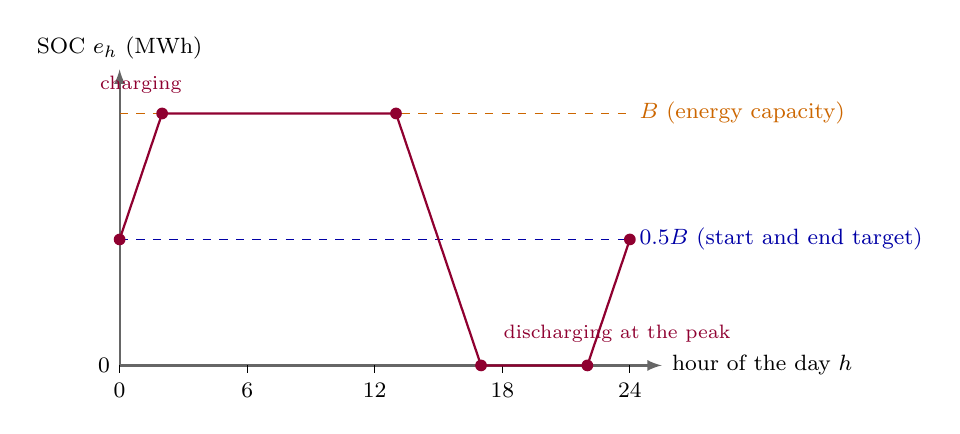
\begin{tikzpicture}[font=\footnotesize, >=latex, x=0.27cm, y=0.8cm]
  % Illustrative hourly SOC path over one representative day with B = 4P:
  % starts and ends exactly at 0.5B, moves by at most P MWh per hour.
  \tikzset{axis/.style={->, thick, draw=gray!80!black},
    point/.style={circle, fill=purple!75!black, inner sep=1.5pt}}
  \draw[axis] (0,0) -- (25.5,0) node[right] {hour of the day $h$};
  \draw[axis] (0,0) -- (0,4.7) node[above] {SOC $e_h$ (MWh)};
  \foreach \h in {0,6,12,18,24} {\draw (\h,0) -- (\h,-0.12) node[below] {\h};}
  \draw[dashed, orange!80!black] (0,4) -- (24,4) node[right] {$B$ (energy capacity)};
  \draw[dashed, blue!65!black] (0,2) -- (24,2) node[right] {$0.5B$ (start and end target)};
  \node[left] at (0,0) {$0$};
  \draw[thick, purple!75!black] (0,2) -- (2,4) -- (13,4) -- (17,0) -- (22,0) -- (24,2);
  \foreach \x/\y in {0/2,2/4,13/4,17/0,22/0,24/2} {\node[point] at (\x,\y) {};}
  \node[font=\scriptsize, text=purple!75!black, align=center] at (1,4.45) {charging};
  \node[font=\scriptsize, text=purple!75!black, anchor=west] at (17.6,0.5) {discharging at the peak};
\end{tikzpicture}
